\documentclass[12pt,twoside,a4paper]{article}
\usepackage[margin=2cm]{geometry}
\usepackage[slantfont,boldfont]{xeCJK}
\usepackage[utf8]{inputenc}
\usepackage{listings}
\usepackage{float}

\setCJKmainfont{PingFang TC}

\title{CV HW1 Report}
\author{林義聖\\B03902048}
\date{}

\usepackage{graphicx}
\graphicspath{ {./} }

\begin{document}

\maketitle

\section{Programming}

\begin{figure}[H]
\centering
\includegraphics[scale=0.4]{lena.bmp}
\caption{original lena picture}
\label{fig:lena.bmp}
\end{figure}

I use \textit{Python} as my programming language and \textit{Pillow} as my Image Library. At first, I read the image in, then load pixel data of the image into Python \textit{list} by calling this function,
\begin{lstlisting}[language=Python]
pixel_data = list(img.getdata())
\end{lstlisting}

\begin{enumerate}

\item
Upside-down the image. The source code of this part is \textit{\textbf{upside-down.py}}.
\begin{lstlisting}[language=Python]
for y in range(height):
  for x in range(width):
    result_data[y*width+x] = pixel_data[(height-y-1)*width+x]
\end{lstlisting}
\begin{figure}[H]
\centering
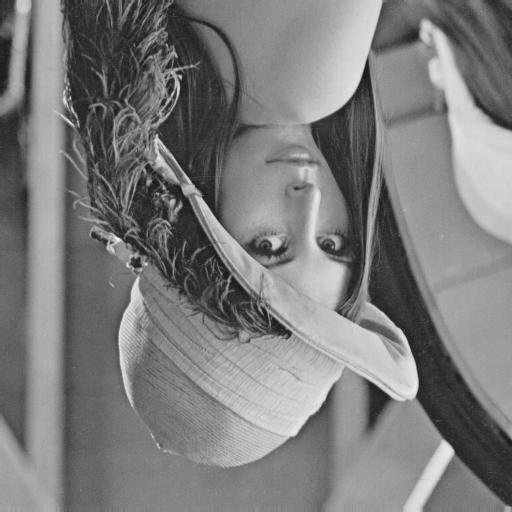
\includegraphics[scale=0.4]{lena-ud.jpg}
\caption{upside-down lena picture}
\label{fig:lena-ud.jpg}
\end{figure}

\item
Right-side-left the image. The source code of this part is \textit{\textbf{right-side-left.py}}.
\begin{lstlisting}[language=Python]
for y in range(height):
  for x in range(width):
    result_data[y*width+x] = pixel_data[y*width+(width-x-1)]
\end{lstlisting}
\begin{figure}[H]
\centering
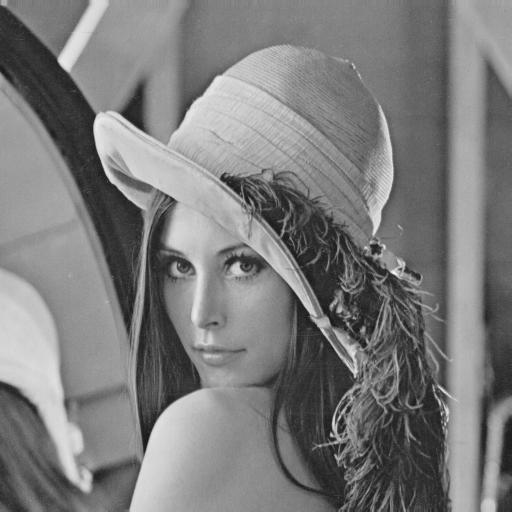
\includegraphics[scale=0.4]{lena-rl.jpg}
\caption{right-side-left lena picture}
\label{fig:lena-rl.jpg}
\end{figure}

\item
Diagonal mirror the image. The source code of this part is \textit{\textbf{diagonal-mirror.py}}.
\begin{lstlisting}[language=Python]
for y in range(height):
  for x in range(width):
    result_data[y*width+x] = pixel_data[x*width+y]
\end{lstlisting}
\begin{figure}[H]
\centering
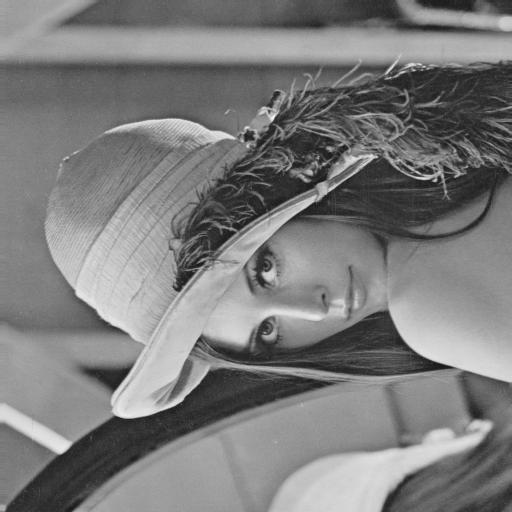
\includegraphics[scale=0.4]{lena-d.jpg}
\caption{diagonal-mirrored lena picture}
\label{fig:lena-d.jpg}
\end{figure}

\end{enumerate}

\section{Image Processing Software}

I use GIMP to manipulate lena.bmp image.

\begin{enumerate}
  \item rotate 45 degrees clockwise\\
    Use rotate tool to rotate image in 45 degrees.
    \begin{figure}[H]
    \centering
    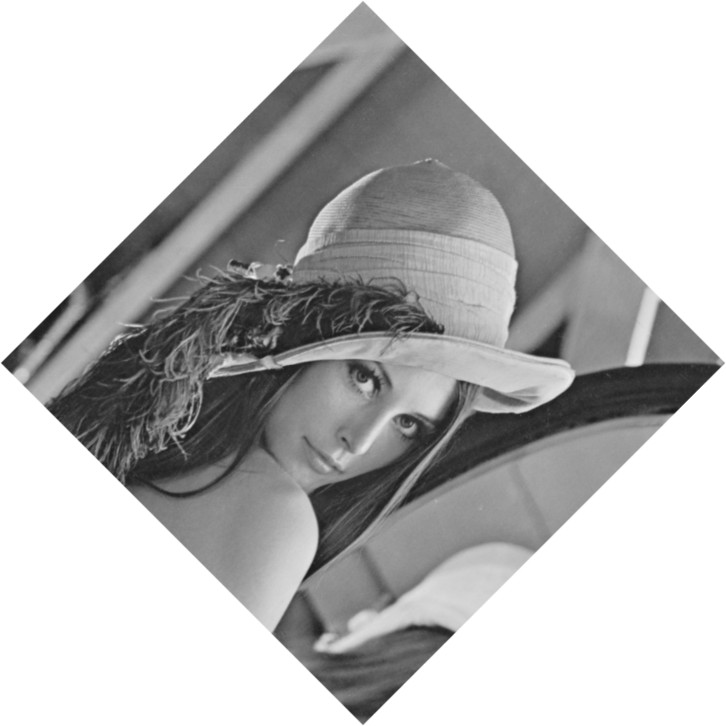
\includegraphics[scale=0.4]{lena-rotated.jpg}
    \caption{rotated lena picture}
    \label{fig:lena-rotated.jpg}
    \end{figure}
      
  \item shrink in half\\
    Use scale tool to scale image from $512 \times 512$ to $256 \times 256$.
    \begin{figure}[H]
    \centering
    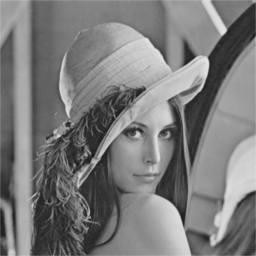
\includegraphics[scale=0.4]{lena-shrinked.jpg}
    \caption{half-shrinked lena picture}
    \label{fig:lena-shrinked.jpg}
    \end{figure}
      
  \item binarize at 128\\
    Use color tool and set up the threshold at 128 to binarized image.
    \begin{figure}[H]
    \centering
    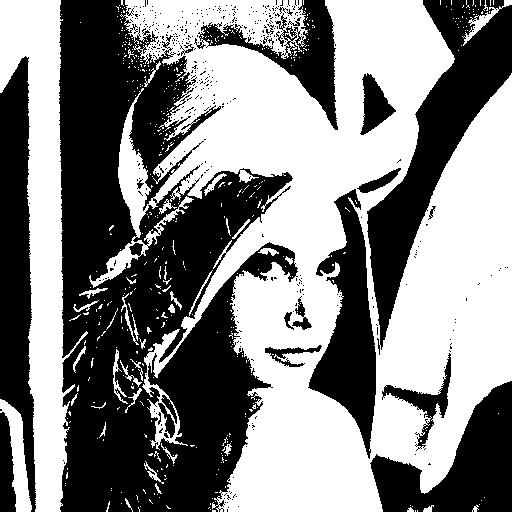
\includegraphics[scale=0.4]{lena-binarized.jpg}
    \caption{binarized lena picture}
    \label{fig:lena-binarized.jpg}
    \end{figure}
\end{enumerate}

\section{How to Use}
For running the three small program (\textit{upside-down.py, right-side-left.py, diagonal-mirror.py}), you need to specify two parameters. The $1^{st}$ is the input image name, and the $2^{nd}$ is the output image name.
\begin{lstlisting}[language=Bash]
> python upside-down.py lena.bmp output.jpg
\end{lstlisting}

\end{document}
